\documentclass[14pt,a4paper]{scrartcl}
\usepackage{cmap}
\usepackage[utf8]{inputenc}
\usepackage[T1,T2A]{fontenc}
\usepackage[english,russian]{babel}
\usepackage{relsize}
\usepackage{graphicx}
\usepackage{subfigure}
\usepackage{mathtools}
\usepackage{amssymb}
\usepackage{float}
\usepackage{sidecap}
\usepackage{wrapfig}
\usepackage{caption}
\usepackage[table,xcdraw]{xcolor}
\usepackage{listings}
\usepackage{minted}
\begin{document}
	\begin{titlepage}
	\begin{center}
		\large
		МИНИСТЕРСТВО ОБРАЗОВАНИЯ И НАУКИ\\ РОССИЙСКОЙ ФЕДЕРАЦИИ
		
		\vspace{0.5cm}
		
		МГТУ им Н.Э.Баумана
		\vspace{0.25cm}
		
		Факультет ФН
		
		Кафедра вычислительной математики и математической физики
		\vfill
		
		
		Соколов Арсений Андреевич\\
		\vfill
		
		
		{\LARGE Домашнее задание №7 по математической статистике\\[2mm]
		}
		\bigskip
		
		3 курс, группа ФН11-53Б\\
		Вариант 9
	\end{center}
	\vfill
	
	\newlength{\ML}
	\settowidth{\ML}{«\underline{\hspace{0.7cm}}» \underline{\hspace{2cm}}}
	\hfill\begin{minipage}{0.4\textwidth}
		Преподаватель\\
		\underline{\hspace{3cm}} Т.\,В.~Облакова\\
		«\underline{\hspace{0.7cm}}» \underline{\hspace{1.71cm}} 2019 г.
	\end{minipage}%
	\bigskip
	
	
	\vfill
	
	\begin{center}
		Москва, 2019 г.
	\end{center}
\end{titlepage}

\section*{Задание 1}


Используя группированную выборку из задачи №1, проверить на уровне $\alpha$ гипотезу $H_0$: выборка взята из генеральной совокупности, распределенной по закону $F(x)$. Неизвестные параметры распределения $F(x)$ найти методом моментов.\\
\textbf{Решение.}\\


Рассмотрим выборку:
\begin{minted}{R}
> df <- read.csv("db.csv", header = F) #data import
> df$V1
[1] 14.495  5.343 14.396 12.888  2.375  9.234
[7]  5.811  4.727  4.843  3.377  8.681 12.173
[13]  4.715 17.985  8.592 10.268 17.921  6.078
[19]  7.241  4.646  9.927 16.195  5.006 17.757
[25]  7.175 15.992  8.206  9.182  9.097  4.964
[31]  5.814 15.535 15.864 12.040  3.608  6.883
[37]  8.428 13.890 14.237  5.647 15.850  6.355
[43]  3.086  9.919  3.635 12.768  2.867  2.666
[49] 11.093  9.838  7.357  8.282 11.449 13.957
[55]  6.875 17.117 17.963  2.744 12.177  9.861
[61]  3.375 13.924 10.821  2.903 11.095 12.911
[67]  3.878 10.351  8.250 14.186 15.506  5.743
[73] 12.906  9.012 12.767 15.988  9.493 15.694
[79]  5.333 16.892  5.140  9.354  7.683 16.175
[85]  8.415  9.458 16.058 12.959 12.175 14.286
[91] 15.134 12.423  6.734 15.439 14.022 15.308
[97]  8.916 17.690 12.959 14.919  7.479  9.869
[103] 12.924 10.511 12.622 14.612 17.103  7.039
[109] 13.480  6.542  4.354  6.339 13.535  5.175
[115]  9.159  4.942 13.325 15.649  8.905 15.238
\end{minted}


Параметры нашего распределения имеют вид:
\begin{align*}
	a = X_{(1)}\\
	b = X_{(120)}
\end{align*}

\begin{minted}{R}
> a <- min(df)
> a
[1] 2.375
> b <- max(df)
> b
[1] 17.985
\end{minted}

Тогда исходная случайная величина имеет непрерывное равномерное распределение на отрезке $[a;b] = [2.375; 17.985]$ и ее плотность $f_X(x)$ имеет вид:

\begin{equation*}
f_X(x) = 
\begin{cases*}
\frac{1}{15.610}, & x $\in$ [2.375; 17.985]  \\
0, & x $\notin$ [2.375; 17.985]. \\
\end{cases*}
\end{equation*}


Рассмотрим нулевую гипотезу $H_0$, заключающуюся в том, что выборка взята из генеральной совокупности, распределенной по равномерному закону, с уровнем доверия $\alpha = 0.01$.


Для проверки выдвинутой гипотезы воспользуемся критерием хи-квадрат: сравним рассчитанные по нашей выборке статистику $\chi^2_B$ с квантилем ${\chi^2_{1-\alpha} (m-1)}$, где $m$ -- число степеней свободы, которое в данном случае равно $m=6$.


Рассчитаем статистику $\chi^2_B = \sum\limits_{i,j} \frac{f_{ij} - e_{ij}}{e_{ij}}$, где ${f_{ij}}$ --  относительные выборочные частоты, а ${e_{ij}}$ -- теоретические частоты:

\begin{minted}{R}
> pt1 <- c(punif(pl1$breaks[2],a,b),
+          punif(pl1$breaks[-c(1:2,length(pl1$breaks))], a,b)
+         - punif(pl1$breaks[-c(1,(length((pl1$breaks))-1):
+                                 length((pl1$breaks)))], a,b))
> pt1
[1] 0.125 0.125 0.125 0.125 0.125 0.125 0.125
> pt <- c(pt1, 1-sum(pt1))
> pt
[1] 0.125 0.125 0.125 0.125 0.125 0.125 0.125 0.125
> npt <- pt * n
> npt
[1] 15 15 15 15 15 15 15 15
> chi_sq <- sum((npt - pl1$counts)^2/(npt))
> chi_sq
[1] 11.06667
\end{minted}

А также квантиль ${\chi^2_{0.99} (5)}$:

\begin{minted}{R}
> qchisq(0.99,5)
[1] 15.08627
\end{minted}

Имеем:
\begin{align*}
11.06667 &< 15.08627 \\
&\rotatebox[origin=c]{-90}{$\Leftrightarrow$} \notag \\ 
\chi^2_B &< {\chi^2_{0.99} (5)}
\end{align*}


Таким образом, у нас нет оснований отвергнуть нулевую гипотезу $H_0$.


Построим гистограмму частот:
\begin{minted}{R}
> png(filename = "../img/hist_with_unif_dens.png", 
+     width = 1920, height = 1080,
+     pointsize = 24, res = 96 * 1.25)
> par(mar = c(3, 3, 2, 1), xaxs = "i", yaxs = "i")
> pl1 <- hist(df$V1,
+             breaks = seq(min_el, max_el, by = bin_width), 
+             xlim = c(0, 20), ylim = c(0.00,0.10), axes = F, freq = F,
+             main = "Histogram of data")
> axis(1, seq(0, 20, 1))
> axis(2, seq(0.00, 0.10, 0.01), las = 1)
> grid(nx = 20, ny = 10, equilogs = F)
> curve(dunif(x, 2.5978, 17.9383), 2.5978, 17.9383, 
+       xlim = c(0,20), add = T, col = "red", lwd = 3)
> legend("topright", c("uniform density"), 
+        lty=c(1), 
+        fill=c("red"))
> dev.off()
\end{minted}

\begin{figure}[h]
	\center{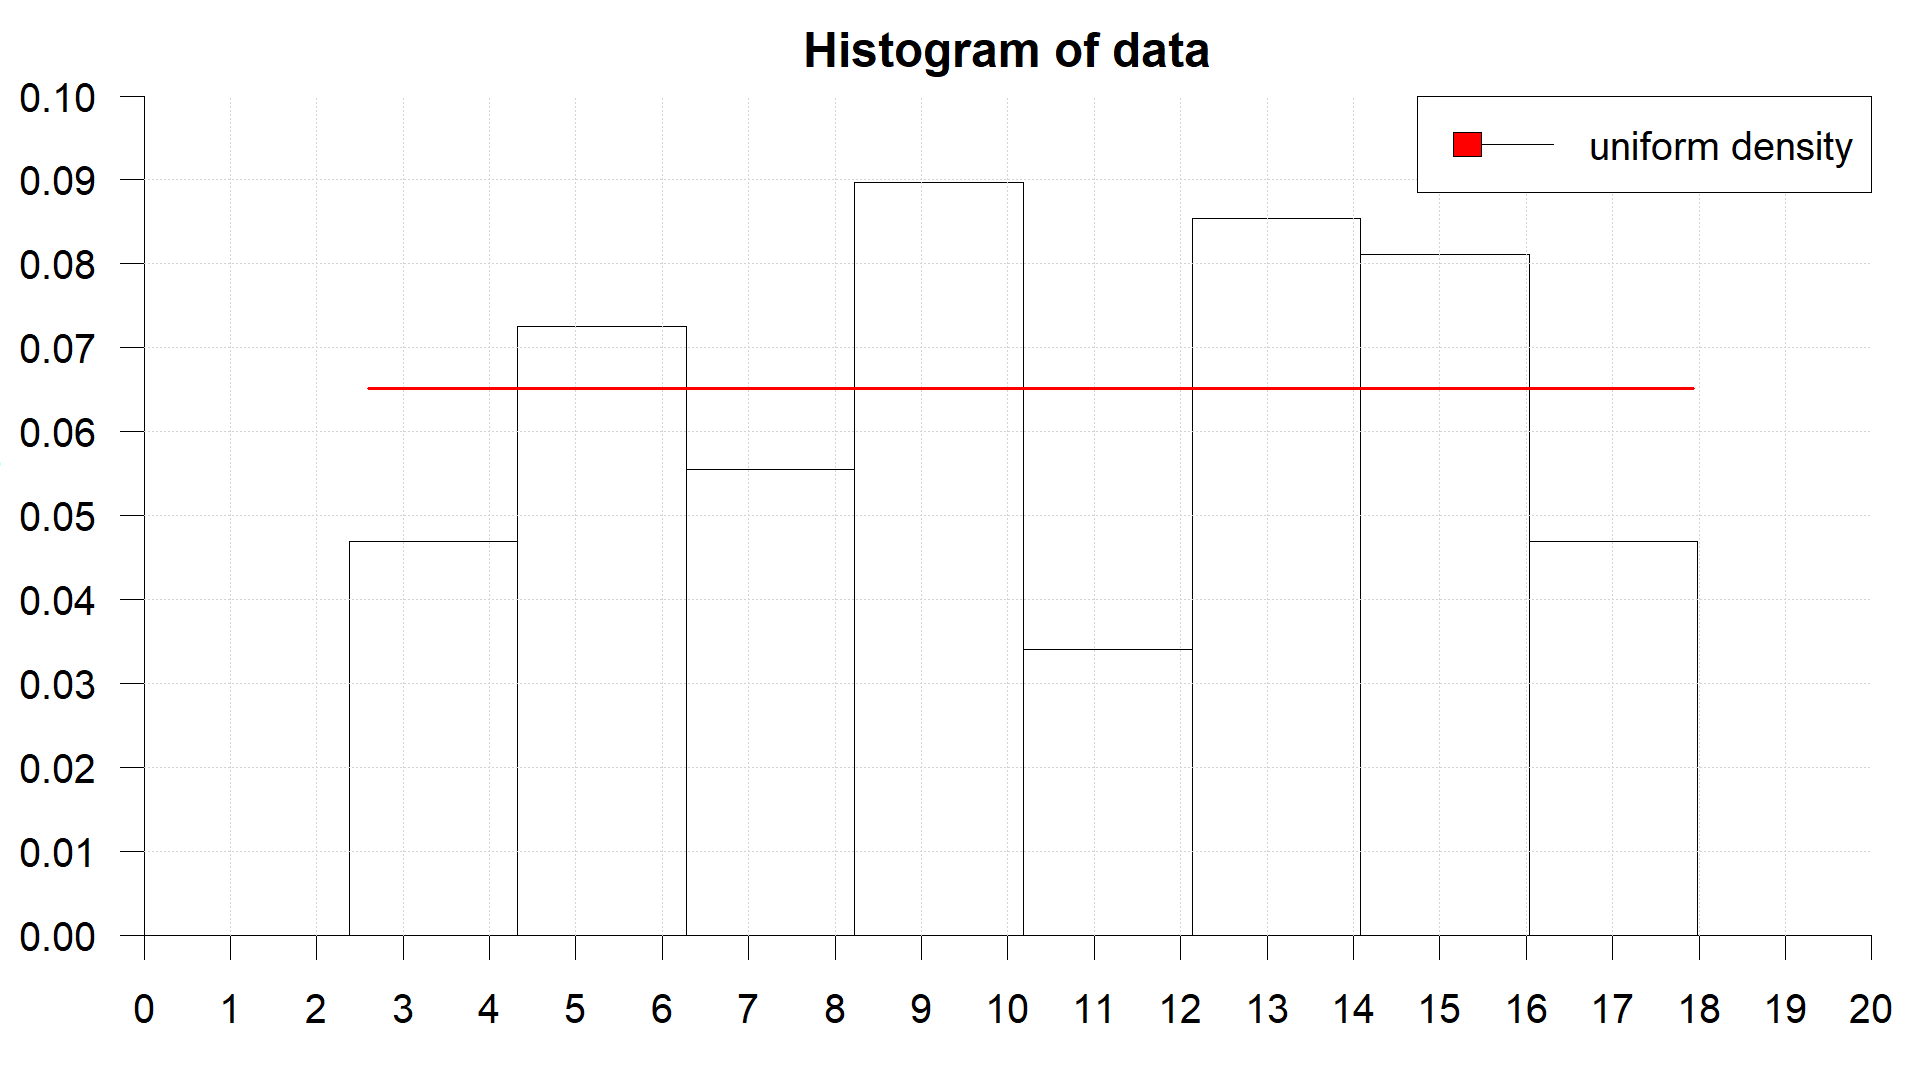
\includegraphics[width=1\linewidth]{../img/hist_with_unif_dens.png}}
	\caption{Совмещённый график гистограммы и плотности равномерного закона.}
	\label{ris:hist_with_unif_dens}
\end{figure}




\end{document}